Blinking two LEDs is easy with \plumbing.

\GOALS
Blink two LEDs together or separately, using the circuit from the previous chapter.

\CODE
\lstinputlisting[caption=We can {\procname blink} in \PARallel.,label=code:blink-par]{code/blink-par.occ}

\PATTERNS

\begin{figure}[h]
  \begin{center}
    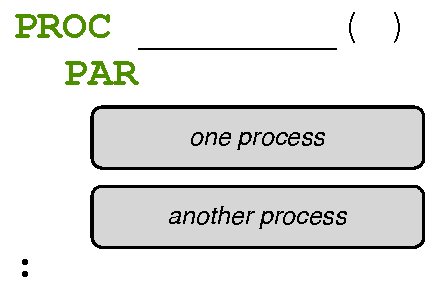
\includegraphics[width=0.6\linewidth]{images/pattern-par}
    \caption{Executing two processes in parallel.}
    \label{pattern:par}
  \end{center}
\end{figure}

In the previous chapters, we've written a {\procname main} procedure that only did one thing. However, interesting programs need to do lots of things {\em at the same time}. If we want two things to happen at the same time, we use \PAR.

So far, we have seen that a \PROC may only contain one process, and that is indented by two spaces. If we want to do two things simultaneously, then we need to use something like a \PAR. Then, indenting two more spaces, we can put {\em any number of additional processes}. In the code in Listing~\vref{code:blink-par}, you can see that we are asking \plumbing to run two things in parallel, because there are two procedures underneath the \PAR.

As it happens, we are asking \plumbing to run two {\procname blink} processes. This is fine, because we're going to ask it to blink the LED on pin {\constant 13} at the same time as we blink the LED on pin {\constant 14}. Type in this new program and upload it to your Arduino; if all goes well, both LEDs should be blinking at the same time.

\subsection{The truth about \PAR}
We have been saying that when you indent processes underneath a \PAR that they will happen ``at the same time.'' This is the real-world implication of things happening ``in parallel.'' However, your Arduino only has one processor, and therefore it can only do one thing at a time.

However, it executes 16 million instructions every second---it is a 16MHz processor, after all. Therefore, we can create the illusion of things happening at the same time by doing them one-after-another very, very quickly. Typically, we refer to this process of letting one process take turns with another as {\em concurrency}. So, to be completely truthful, we should say that everything that you indent underneath a \PAR will run concurrently---everything will get a turn. Now you might begin to understand why our projects are hosted under the URL \url{http://concurrency.cc/}.

When you write programs that use \PAR, things aren't truly happening ``at the same time.'' However, \plumbing is doing a lot of hard work for you to make sure that it {\em looks like} things are happening at the same time. This is what makes \plumbing different from any other environment you might use on your Arduino.

\EXPLORATIONS
There isn't much else to say in this chapter; you've just learned how to blink two LEDs at the same time (or so they appear to blink at the same time). You should be able to do some additional explorations on your own, at this point.

\begin{description}
	\item[Vary the parameters]\ \\
	Currently, both LEDs are blinking at the exact same rate. Try changing the rate at which they blink by varying the second parameter to the {\procname blink} process.
	\item[Add more LEDs]\ \\
	If you have more LEDs, you should be able to wire them up like your first LED using more pins on the Arduino. Then, add more {\procname blink} processes underneath the \PAR that will turn that pin on and off.
\end{description}

\BREAKAGE
There are a lot of neat ways to break the code in this chapter.

\begin{description}
		\item[Indentation of \PAR]\ \\
	What happens if you fail to indent \PAR, but indent all of the {\procname blink} procedures? This is a very common error.
		\item[Lowercase \PAR]\ \\
	What happens if you make {\bfseries par} all lowercase? Partially lowercase? This is another common error.
	\item[Indentation of {\procname blink}]\ \\
	Try indenting each {\procname blink} process two spaces more than it is now. What happens?
	\item[Multiple {\procname blink}s on one pin]\ \\
	Modify your program so that two of your {\procname blink} processes refer to the same pin number. Note that this is an error that is only detected {\em after} you upload your program!
	\item[Replace one {\procname blink} with a {\procname heartbeat}]\ \\
	Modify your program so the \PAR looks like this:
	\begin{lstlisting}[firstnumber=2]
PAR
  heartbeat ()
  blink (14, 500)
	\end{lstlisting}
	What happens? Does this break anything? Why or why not?
	\item[Replace another {\procname blink} with a {\procname heartbeat}]\ \\
	Modify your program so the \PAR looks like this:
	\begin{lstlisting}[firstnumber=2]
PAR
  blink (13, 500)
  heartbeat ()
	\end{lstlisting}
	What happens? Does this break anything? Why or why not?
\end{description}
	
